\chapter{Computational Details}
\label{cha:comp}

\section{2D Test Potentials}
\label{sec:comp 2D}
For test purposes we consider a single particle of mass $10$~a.u. moving in two-dimensional potentials of the form
\begin{equation}
  U_1(x,y) = a(x-c)^2(x+d)^2 + by^2 \label{eq:U1}
\end{equation}
\begin{equation}
  U_2(x,y) = -\ln\bigl( e^{-a(x+c)^2 - b(y-d)^2} + e^{-a(x+c)^2 - b(y+d)^2} \bigr) \label{eq:U2}
\end{equation}
where $x,y$ are particle coordinates and $a,b,c,d$ are parameters of the potentials given in table~\ref{tab:2D pots} of the appendix, respectively.
\begin{figure}[H]
    \centering
    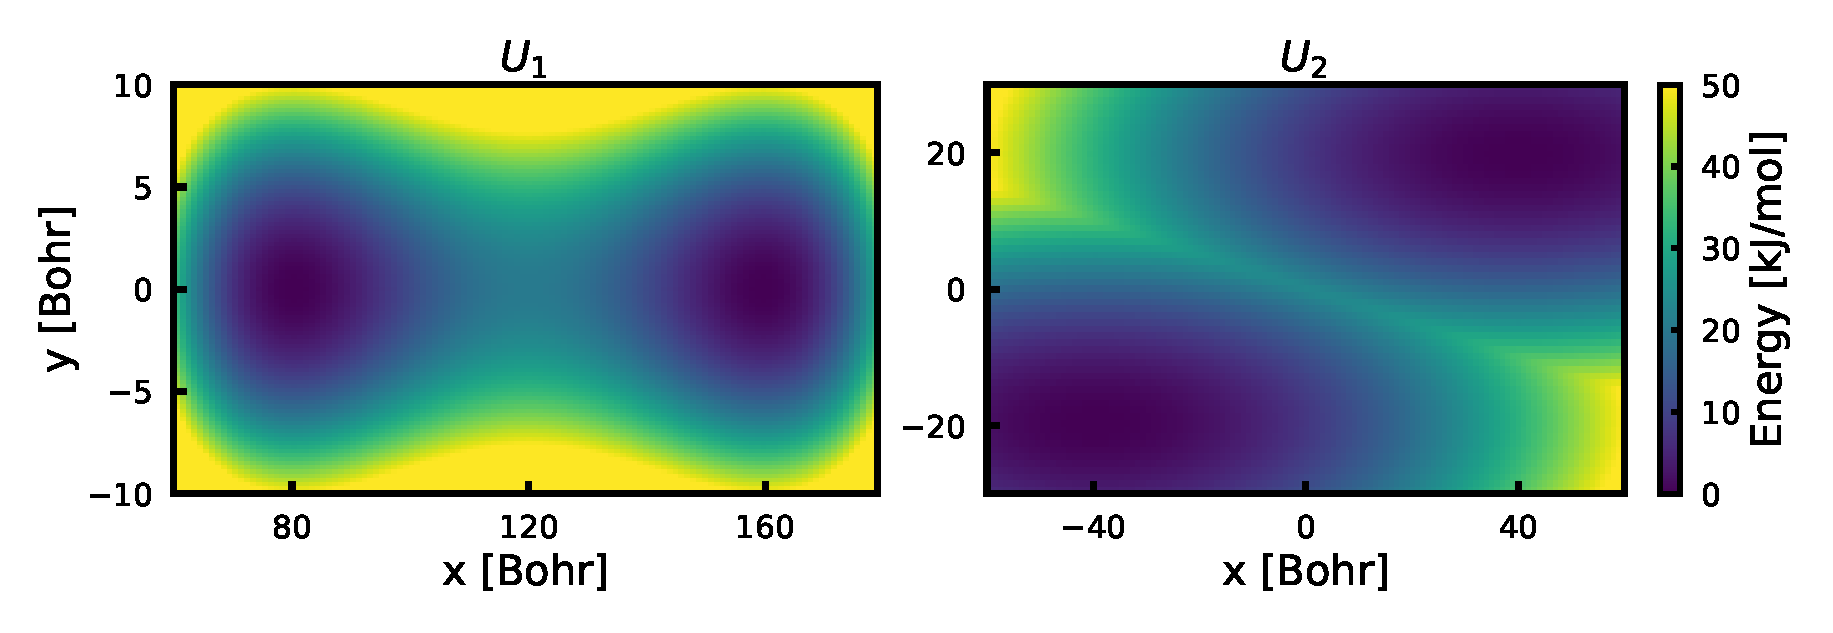
\includegraphics[width=1.0\textwidth]{bilder/U}
    \caption{Potentials for test calculations, Minima of $U_1$ are at located at (80,0) and (160,0). Minima of $U_2$ are located at (-40,-20) and (40,20). In both potentials minima are separated by free energy barriers of $20$~kJ/mol.}
\label{fig:potentials}%
\end{figure}
To simulate the particles dynamics a Velocity Verlet\autocite{swope1982computer} integrator is applied with a time step of 5~fs.
The initial momenta are drawn randomly from a Maxwell-Boltzmann distribution at 300~K.
Afterwards the temperature is controlled at 300~K by a Langevin thermostat\autocite{kroger2005models} with friction constant 0.001~fs$^{-1}$.
Crucial to the metastability of the system is the ratio of thermal energy~$k_B T$ to the barrier height.
Here, we always use transition barriers of height 8~$k_B T$ (20~kJ/mol).
Spontaneous transitions between minima in unbiased simulations can therefore be expected to be rare events.
All test simulation are completely performed in Python.

\section{Molecular Dynamics Simulations}
\label{sec:comp MD}
For QM simulations a Python interface for the in-house program suite FermiONs++\autocite{} was used.
Propagation of atomic coordinates with the Velocity Verlet\autocite{swope1982computer} integrator and temperature control with the Langevin thermostat\autocite{kroger2005models} (see algorithm~\ref{alg:ABM}) is done in Python.
For QM energy and gradient evaluation the PyFermiONsInterface was used.
All systems are simulated in vacuum.
To generate starting structures for MD simulations minimum energy geometries are obtained with the FermiONs intern geometry optimizer. MD simulations always consist of the following three steps:
\begin{enumerate}
  \item \textit{Heating}: Simulations are heated from 1~K to 300~K in 3000 time steps with a step size of 0.1~fs. Initial momenta are randomly drawn from a Maxwell-Boltzmann distribution. The velocities are rescaled every 10~time steps to increase the temperature by 1~K.
  \item \textit{Equillibration}: For thermal equilibration of the heated system is simulated for 1.0~ps under application of the Langevin thermostat at 300~K with a friction coefficient of 0.001~fs$^{-1}$. The time-step is increased to 0.5~fs. To produce starting structures for free energy estimation the system is also confined to the range of interest in CV space with harmonic walls.
  \item \textit{Production}: For production runs the equilibrated system is simulated under additional application of some enhanced sampling algorithm (see section~\ref{sec:comp ABM}).
\end{enumerate}

\section{Adaptive Biasing Implementation}
\label{sec:comp ABM}
All biasing algorithms are implemented in Python under extensive use of NumPy\autocite{harris2020array} and the PyFermiONsInterface.
For all methods the range of interest in CV space ($\xi_{min},\xi_{max}$), as well as the bin width $\Delta\xi$ are input parameters.
Simulations are restraint to this range by harmonic walls of the form
\begin{equation}
U^c(\xi) =\left\{\begin{array}{ll} \frac{k^c}{2}\bigl(\xi(\textbf{x}) - \xi^c_{min} \bigr)^2, & \xi \leq \xi^c_{min} \\
                                   \frac{k^c}{2}\bigl(\xi(\textbf{x}) - \xi^c_{max} \bigr)^2, & \xi \geq \xi^c_{max} \\
                                    0, & \text{otherwise}
          \end{array}\right.
\label{eq:harmonic wall}
\end{equation}
with restraining force constant $k^c$ and boundary of the simulation $\xi^c$.
For all simulations a stiff restraining force constant of $k^c=1000$~kJ/(mol$\Delta\xi^2$) is applied. The choice of boundaries ($\xi^c_{min}$,$\xi^c_{max}$) depends on the specific method and will be discussed in the following sections.
Probability distributions and free energy estimates are computed on fixed grids of the form ($f(\xi_{min}),f(\xi_{min}+\Delta\xi),...,f(\xi_{max})$).
All algorithms are computationally lightweight compared to QM energy and force evaluations and their impact on the overall computation time is negligible.

\subsection{MtD/WTM}
\label{subsec:implement MtD}
MtD/WTM potentials are accumulated on grids and free energy estimates obtained from equations~\ref{eq:F est MtD}/\ref{eq:F est WTM} are written to an output file in fixed intervals.
For MtD the height and variance of Gaussian hills $W$ and $\sigma_G$, as well as frequency of hill creation $\tau_G$ are input parameters. For WTM additionally $\Delta T$ is chosen to control how fast the Gaussian height decreases. Default parameters are given in table~\ref{tab:metaparams}.
\begin{table}[H]
      \centering
         \caption{Default parameters for MtD/WTM simulations.}
         \begin{tabular}{ c  c }
                 \hline
                  $\sigma_G$  & -        \\
                  $W$         & 1~kJ/mol \\
                  $\tau_G$    & 10~fs    \\
                  $\Delta T$  & 2000~K   \\
                 \hline
      \end{tabular}
      \label{tab:metaparams}
\end{table}
The MtD/WTM bias forces given by derivatives of eq.~\ref{eq:U_mtD}/\ref{eq:WTM} are also summed together and saved on a grid between update times of the potential.
In long simulations this is much more efficient than evaluating each hill at every step and yields negligible errors.\autocite{fiorin2013using}
The boundaries for the confinement of the simulation are set to
$\xi^c_{min}=\xi_{min}+2\Delta\xi$ and $\xi^c_{max}=\xi_{max}-2\Delta\xi$ for the lower and higher boundary, respectively, to avoid that the system is pushed out of the grid by the repulsive MtD/WTM potential.
To avoid that the bias forces suddenly vanish at the boundary they are calculated from hill centers near the margin, if the system still leafs the grid.
The resulting PMF will show a sharp increase at the margin, where the wall potential kicks in.

\subsection{ABF, eABF and WTM-eABF}
For ABF calculations two accumulators are used to store the biased histogram and sum of instantaneous force samples. The mean force is evaluated according to eq.~\ref{eq:mean force}.
The only ABF specific input parameter is the number of samples $N_{full}$ given to ramp function~\ref{eq:ramp}.
Force samples are calculated by eq.~\ref{eq:inst ABF force} and the inverse gradient is always chosen as $\textbf{v}_i = \nabla \xi_i/|\nabla \xi_i|^2$. Expressions for the divergence of $\textbf{v}_i$ for all applied CVs are given in the Appendix.
Constraints~\ref{eq:cond1} and \ref{eq:cond2} have to be fulfilled by choice of CV.
Harmonic walls are used to constrain the system to the range of interest.
Since the ABF force is not repulsive it is sufficient to apply the restraining force directly at the margin of the grid ($\xi^c_{min}=\xi_{min}$, $\xi^c_{max}=\xi_{max}$).

A flowchart of the full eABF/CZAR algorithm is given in figure~\ref{fig:eABF flowchart}.
The mass of the fictitious particle $m_\lambda$ and force constant $k_\lambda$ of its harmonic coupling to the physical system are free parameters.
Instead of directly choosing $k_\lambda$ the \textit{thermal width} of coupling $\sigma_\lambda$ is used as input parameter, which determines $k_\lambda$ by the following expression:
\begin{equation}
  k_\lambda = \frac{1}{\beta \sigma^2}
\end{equation}
The propagation of fictitious particles with a Velocity-Verlet\autocite{swope1982computer} integrator and temperature control by a Langevin thermostat\autocite{kroger2005models} is done completely independent of the physical system, but always using the same parameters.
$\xi$-conditioned expressions for CZAR are stored independently of $\lambda$-conditioned expressions for the eABF bias and CZAR estimates for the thermodynamic force on $\xi$ are computed at output times.
Additionally CZAR can be evaluated from trajectories of $\xi$ and $\lambda$ after the simulation has finished.
This way enhanced sampling and free energy estimation are completely independent.
MtD/WTM potentials and forces for (meta/WTM)-eABF are calculated as described in section~\ref{subsec:implement MtD} and eABF forces are accumulated separately.
Boundaries for the confinement of $\lambda$ are set to $\xi^c_{min}=\xi_{min}+2\sigma_\lambda$ and $\xi^c_{max}=\xi_{max}-2\sigma_\lambda$ for the lower and higher boundary, respectively. This way save confinement of $\xi$ to the region of interest is ensured only by its coupling to $\lambda$.

For 1D CVs PMFs are obtained at output times by numerically integrating the ABF or CZAR estimates of the thermodynamic force with the rectangular rule.\autocite{davis2007methods}
To generate 2D PMFs force estimates for both dimensions are stored and integrated separately with the FEM method.
For this purpose four control points are obtained between original data points by linear interpolation. The RMSD between B-spline functions and control points (eq. \ref{eq:RMSD}) is than minimized with the Broyden–Fletcher–Goldfarb–Shanno (BFGS) algorithm.\autocite{nocedal2006numerical}

\begin{figure}[H]
   \caption{
     Flowchart of the eABF algorithm. $k_{\lambda}$ and $k_\xi$ denote $\lambda$ or $\xi$ conditioned bin indices, respectively, in bins with size $\Delta\xi$. $P^B_\lambda$ and $P^B_\xi$ are $\lambda$- or $\xi$- conditioned histograms and $R$ is the ABF ramp function. $F_B$ is the sum of force samples. Outputs are written in fixed intervals.
   }

        \centering
        \begin{tikzpicture}[minimum size=5mm,node distance=4cm and 7cm,>=stealth,bend angle=45,auto]
        \node [block] (xi) {$\xi \leftarrow f(\textbf{x})$};
        \node [block, below of=xi] (langevin) {Langevin dynamics of extended system};
        \node [block, below of=langevin,yshift=-0.5cm] (F_ext) {add harmonic force of extended system to QM/MM forces};

        \node [decision, below of=F_ext, yshift=-1cm] (decide_lambda) {$\xi_{min}\leq \lambda \leq \xi_{max}$};

        \node [block, below of=decide_lambda,xshift=-3cm] (la_bin) {$k_\lambda = \lfloor \frac{|\lambda - \xi_{min}|}{\Delta \xi} \rfloor$};
        \node [block, below of=la_bin] (la_hist) {$P^B_\lambda(k_\lambda) \pluseqq 1$};
        \node [block, below of=la_hist] (R) {$R(k_\lambda) = f(k_\lambda)$ (eq. \ref{eq:ramp})};
        \node [block, below of=R] (F_B1) {$\overline{F}_B(k_\lambda)=\frac{(\lambda_i-\braket{\xi_i}_{\lambda_i})}{\sigma_i^2}$};
        \node [block, below of=F_B1] (F_B2) {$\textbf{F}(\textbf{x},\lambda) \pluseqq R(k_\lambda)\overline{F}_B(k_\lambda)\nabla\lambda$};

      %  \node [block, right of=R,xshift=4cm] (conf1) {confine $\lambda$ to range of interest};

        \node [decision, below of=F_B2,xshift=3cm] (decide_xi) {$\xi_{min}\leq \xi \leq \xi_{max}$};

        \node [block, below of=decide_xi,xshift=-3cm] (xi_bin) {$k_\xi = \lfloor \frac{|\xi - \xi_{min}|}{\Delta \xi} \rfloor$};
        \node [block, below of=xi_bin] (xi_hist) {$P^B_\xi(k_\xi) \pluseqq 1$};
        \node [block, below of=xi_hist] (F_corr) {$\overline{F}_{corr}(k_\xi)=\frac{(\braket{\lambda_i}_{\xi_i}-\xi_{i})}{\sigma_i^2}$};

      %  \node [block, right of=xi_hist,xshift=4cm] (conf2) {confine $\xi$ to range of interest};

        \node [block,below of=F_corr,xshift=3cm,yshift=-0.5cm] (MD1) {Finish Langevin dynamics of extended system};

        \node [decision, left of=decide_xi,xshift=-5.5cm] (output) {write output?};
        \node [block, left of=F_B1,xshift=-6cm] (CZAR) {calculate CZAR according to eq. \ref{eq:CZAR}};
        \node [block, left of=la_bin,xshift=-6cm] (out) {write output};

        \node [block, above of=output,yshift=10cm] (MD2) {MD step of physical system. (compare Algorithm \ref{alg:ABM})};

        \path [line] (xi) -- (langevin);
        \path [line] (langevin) -- (F_ext);
        \path [line] (F_ext) -- (decide_lambda);

        \path [line] (decide_lambda) -- node [above,xshift=-0.3cm] {yes} (la_bin);
        \path [line] (la_bin) -- (la_hist);
        \path [line] (la_hist) -- (R);
        \path [line] (R) -- (F_B1);
        \path [line] (F_B1) -- (F_B2);

        \draw [->] (decide_lambda) -- node {no} (decide_xi);

        \path [line] (F_B2) -- (decide_xi);
      %  \path [line] (conf1) -- (decide_xi);

        \draw [->] (decide_xi) -- node [above,xshift=-0.3cm] {yes} (xi_bin);
        \path [line] (xi_bin) -- (xi_hist);
        \path [line] (xi_hist) -- (F_corr);

%\draw [->] (decide_xi) -- node {no} (conf2);

        \path [line] (F_corr) -- (MD1);
        \path [line] (decide_xi) -- node [right] {no} (MD1);

        \path [line] (MD1) -| (output);
        \path [line] (output) -- node [below,yshift=-0.2cm] {yes} (CZAR);
        \path [line] (CZAR) -- (out);
        \path [line] (out) -- (MD2);

        \draw[->] (output) -- node [right] {no} (MD2);
        \draw[->] (MD2) |- (xi);

        \end{tikzpicture}
        \label{fig:eABF flowchart}
\end{figure}
